\begin{figure}[ht]
	\centering
	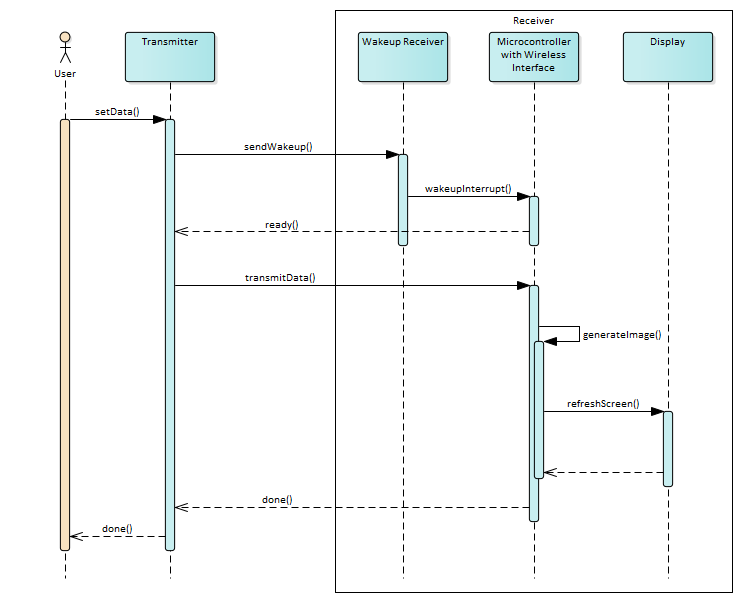
\includegraphics[width=0.9\textwidth]{4-development/software/graphics/1.png}
	\caption{not up to date sequence\label{software:sequence}}
\end{figure}

The software of the ULPWUR is separated in three different parts. 

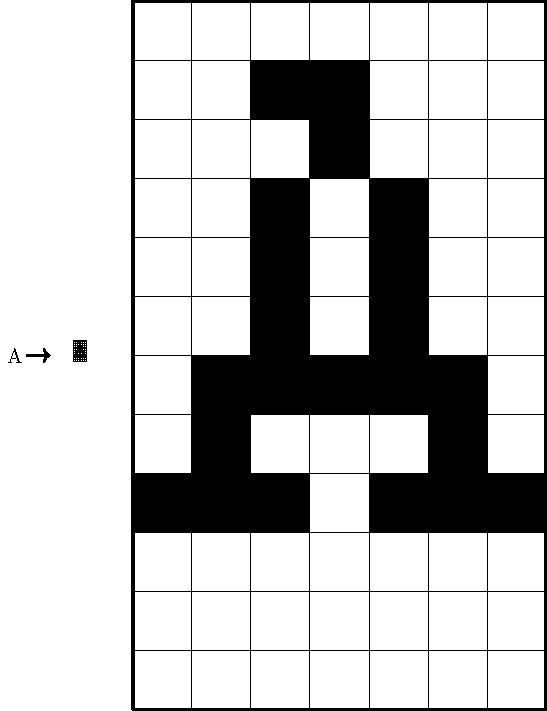
\includegraphics[scale=0.3]{4-development/software/graphics/font12.pdf}

\subsection{Receiver}

\subsubsection{Python-script}
\lstset{basicstyle=\footnotesize}
\lstdefinestyle{mystyle}{
	language=Python,
	basicstyle=\footnotesize\ttfamily,
	morekeywords={as},
	keywordstyle=\color{blue!50!black},
	stringstyle=\color{green!50!black},
	numberstyle=\color{red},
	emph={int,char,double,float,range, len},
	emphstyle=\color{violet}
}
\lstset{style=mystyle}

A short python script enables the user to send the data over an USB-port to the nRF52840.

%\lstinputlisting{4-development/software/code/WriteSection.py}

\subsubsection{nRF52840}
The software on both sides of the bluetooth channel is very similar, thus it is explained in this section.
A \acs{ble} example project, which was provided by nordic, was only slightly changed to fit the purpose of this prototype.

Before a connection is established, the module on the receiver side is known as peripheral, and the module on transmitter end as the central device.
After the receiver is woken up with the RFicient, the peripheral starts advertising.
Advertising basically means sending data packets periodically with information for the central device.
The central is scanning for the this advertisement and can based on this information decide, if it wants to connect.
Is the connection established, it is now possible to exchange data through this channel.
This process is illustrated in figure \ref{software:ble}.
\begin{figure}[ht]
	\centering
	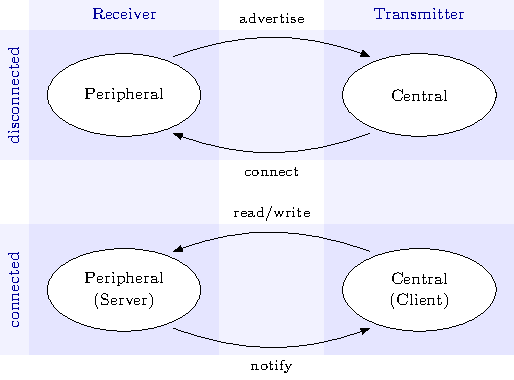
\includegraphics[width=0.9\textwidth]{4-development/software/graphics/ble.pdf}
	\caption{\acs{ble}-communication with the nRF52480\label{software:ble}}
\end{figure}

The central serves after connection as the client.
It can make read and write requests to access the data on the peripheral, which acts as the server.
The server on the other hand can only send notifications to the client if new data is ready.
It should be noted, that the roles of client and server do not in any case have to be assigned to the central and peripheral, but also the other way around. 

\subsection{Transmitter}